\chapter{Analyse et spécification des besoins}
\begingroup
\etocsettocstyle{\rule{\linewidth}{\tocrulewidth}\vskip0.5\baselineskip }{\rule{\linewidth}{\tocrulewidth}}
\localtableofcontents
\endgroup
\newpage
\section{Introduction}
 Après avoir défini le périmètre fonctionnel et établi la planification stratégique dans le chapitre précédent, nous abordons maintenant la phase d'analyse et de spécification technique qui transforme les besoins identifiés en architecture logicielle concrète. Ce chapitre constitue le pont essentiel entre les exigences métier et l'implémentation technique, en structurant notre vision à travers des modèles architecturaux et des diagrammes UML précis.

Nous présentons d'abord l'architecture logicielle retenue, basée sur le pattern MVC qui sépare clairement les responsabilités tout en facilitant l'intégration des modules d'intelligence artificielle. Ensuite, nous détaillons l'architecture globale du système avec ses composants principaux et leurs interactions. Enfin, nous formalisons la conception détaillée à travers une modélisation UML complète incluant diagrammes de cas d'utilisation et diagramme de classes, offrant ainsi une vision structurée et partagée qui guidera l'implémentation des releases .
\section{Architecture logicielle}
Nous avons opté pour le modèle d'architecture \textbf{MVC}  qui nous permet de structurer clairement notre application en séparant les responsabilités. Cette approche s'avère particulièrement adaptée à notre contexte de développement mobile avec modules d'IA intégrés.

\subsection{Architecture MVC}
\begin{itemize}
    \item \textbf{Modèle (Model)} : Gère toutes les données de l'application (profils utilisateurs, mesures physiologiques, historique des conversations, résultats d'analyses IA) et orchestre l'accès à la base de données MongoDB.
    \item \textbf{Vue (View)} : Représente l'interface utilisateur React Native, incluant les écrans d'authentification, le tableau de bord personnalisé, l'interface de chat avec l'assistant, et les visualisations de données.
    \item \textbf{Contrôleur (Controller)} : Coordonne les interactions entre la vue et le modèle, traite les requêtes utilisateur, sollicite les modules d'IA (rPPG, détection d'émotions, recommandations) et formate les réponses.
\end{itemize}

\subsection{Flux d'interaction }
Le parcours utilisateur s'articule autour de ce modèle : l'utilisateur interagit avec la \textbf{Vue} mobile pour soumettre une image ou envoyer un message, le \textbf{Contrôleur} backend traite la requête en sollicitant les modules d'IA appropriés et met à jour le \textbf{Modèle}, puis les résultats personnalisés sont renvoyés à la vue pour afficher. Cette séparation claire facilite la maintenance et permet une évolution agile de chaque composant.~\cite{MVC}

\begin{figure}[H]
    \centering
    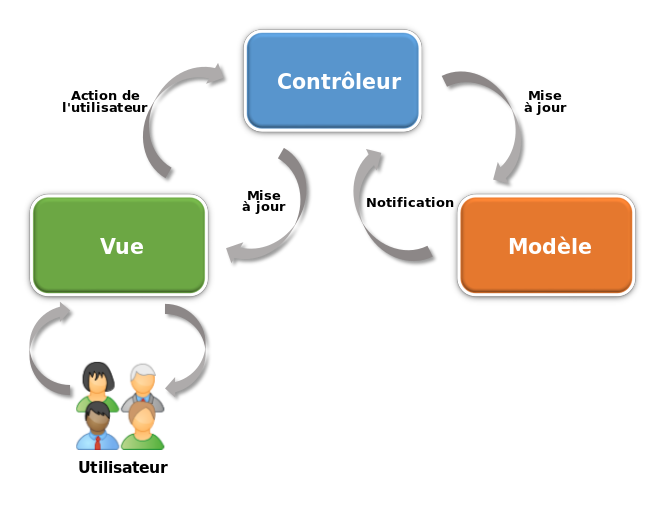
\includegraphics[width=0.8\textwidth]{Figures/Modèle–Vue–Contrôleur.png}
    \caption{Architecture MVC }
\end{figure}

\section{Architecture globale}
Notre architecture globale privilégie une approche modulaire qui sépare clairement les responsabilités tout en facilitant l'intégration harmonieuse des différents composants d'intelligence artificielle.

\subsection{Composants principaux du système}
Le système MindCare-AI s'articule autour de quatre modules principaux :
\begin{itemize}
    \item \textbf{Application mobile React Native} : Interface utilisateur moderne offrant authentification, capture d'images, chat intelligent, et visualisations personnalisées.
    \item \textbf{API REST Node.js/Express} : Serveur backend qui orchestre la logique métier, gère l'authentification JWT, coordonne les appels aux modules d'IA, et assure la persistance des données.
    \item \textbf{Modules d'intelligence artificielle }: 
    \begin{itemize}
        \item Module rPPG pour l'estimation des signes vitaux par analyse d'image faciale.
        \item Analyseur d'émotions pour la classification des sentiments dans les textes.
        \item Assistant conversationnel adaptatif avec génération de réponses empathiques.
        \item Système de recommandations personnalisées basé sur l'état psychophysiologique.
    \end{itemize}
    \item \textbf{Base de données } : Stockage sécurisé et structuré des profils utilisateurs, mesures physiologiques, conversations, et historiques d'analyses.
\end{itemize}

\subsection{Schéma d'architecture}
\begin{center}
\begin{tikzpicture}[node distance=2cm, auto]
    % Nodes
    \node[draw, rectangle, fill=blue!10] (mobile) {Application mobile};
    \node[draw, rectangle, right=4cm of mobile, fill=green!10] (backend) {Serveur backend (API REST)};
    \node[draw, rectangle, above=1.5cm of backend, fill=yellow!10, align=center] (ai) {Modules IA\\(vital\_signs, chatbot, émotions)};
    \node[draw, rectangle, below=1.5cm of backend, fill=red!10] (db) {Base de données (MongoDB)};
    % Edges
    \draw[->, thick] (mobile) -- node[above]{Requêtes API} (backend);
    \draw[->, thick] (backend) -- node[right]{Appels internes} (ai);
    \draw[->, thick] (backend) -- node[right]{Lecture/écriture} (db);
    \draw[<-, thick] (backend) -- node[below]{Réponses API} (mobile);
\end{tikzpicture}
\end{center}

\section{Conception détaillée : langage UML}
La modélisation UML nous a accompagnés tout au long de la conception pour structurer et clarifier les interactions complexes de notre système intégrant à la fois l'analyse physiologique par IA et l'accompagnement conversationnel personnalisé.~\cite{uml}

\begin{figure}[H]
    \centering
    
\includegraphics[width=0.8\textwidth]{Figures/UML_logo.png}
    \caption{ langage de modélisation unifié}
\end{figure}
\subsection{Diagramme de cas d'utilisation global}
Ce diagramme illustre l'ensemble des interactions possibles entre l'utilisateur et notre système intelligent, mettant en évidence la richesse fonctionnelle de MindCare-AI et les relations entre les différents cas d'utilisation.

\begin{figure}[H]
    \centering
    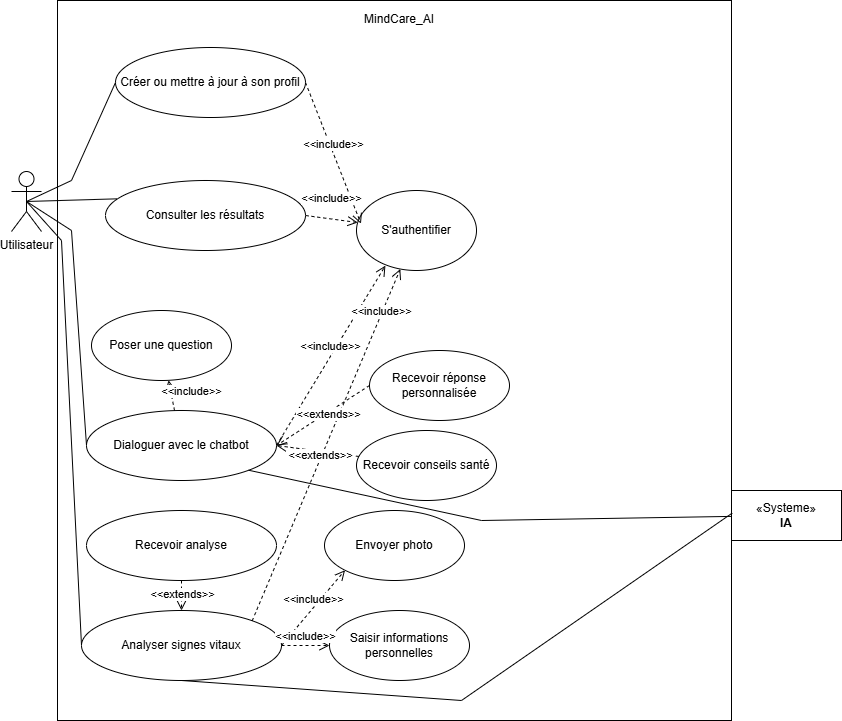
\includegraphics[width=1.1\textwidth]{Figures/useCase.png}
    \caption{Diagramme de cas d'utilisation global }
\end{figure}

\subsubsection*{Description détaillée du diagramme de cas d'utilisation}

\begin{table}[H]
\centering
\small
\begin{tabularx}{\linewidth}{|p{4cm}|X|}
\hline
\textbf{Titre} & Système MindCare-AI \\
\hline
\textbf{Acteur(s)} & Utilisateur \\
\hline
\textbf{Description} & 
Le système MindCare-AI offre un ensemble complet de fonctionnalités pour l'accompagnement en santé mentale. L'utilisateur peut gérer son profil, analyser ses signes vitaux via rPPG, dialoguer avec un assistant conversationnel empathique, consulter son historique avec visualisations, et recevoir des recommandations personnalisées de bien-être. \\
\hline
\textbf{Préconditions} & 
\begin{itemize}
    \item L'application mobile est installée sur le smartphone de l'utilisateur.
    \item L'utilisateur dispose d'une connexion internet active.
    \item Pour l'analyse rPPG : l'appareil dispose d'une caméra fonctionnelle et d'un éclairage suffisant.
\end{itemize} \\
\hline
\textbf{Postconditions} & 
\begin{itemize}
    \item L'utilisateur est authentifié et peut accéder à toutes les fonctionnalités de l'application.
    \item Toutes les données générées (analyses, conversations, évaluations) sont sauvegardées dans l'historique personnel.
    \item L'utilisateur peut consulter ses tendances et évolutions via des visualisations graphiques.
    \item Le système adapte continuellement ses recommandations en fonction de l'état psychophysiologique détecté.
\end{itemize} \\
\hline
\textbf{Scénario principal} & 
\begin{enumerate}
    \item L'utilisateur lance l'application et s'authentifie.
    \item L'utilisateur configure son profil avec ses informations personnelles.
    \item L'utilisateur accède au tableau de bord principal.
    \item L'utilisateur sélectionne une fonctionnalité (analyse des signes vitaux, dialogue avec le chatbot, ou consultation des résultats).
    \item Le système traite la demande et retourne les résultats appropriés.
    \item L'utilisateur reçoit des recommandations personnalisées selon son état détecté.
    \item Les données sont sauvegardées pour un suivi ultérieur.
\end{enumerate} \\
\hline
\end{tabularx}
\end{table}

\begin{table}[H]
\centering
\small
\begin{tabularx}{\linewidth}{|p{4cm}|X|}
\hline
\textbf{Scénarios alternatifs} & 
\begin{itemize}
    \item Échec d'authentification : affichage d'un message d'erreur et possibilité de réessayer.
    \item Problème technique (détection faciale, communication IA, connexion) : affichage d'un message d'erreur explicatif avec proposition de réessai.
    \item Données insuffisantes : le système invite l'utilisateur à effectuer une première analyse ou à compléter son profil.
    \item Résultats avec faible niveau de confiance : le système affiche un avertissement et suggère de refaire l'analyse dans de meilleures conditions.
\end{itemize} \\
\hline
\end{tabularx}
\caption{Description générale du diagramme de cas d'utilisation global}
\end{table}


Cette organisation modulaire et cohérente garantit une expérience utilisateur fluide tout en préparant l'intégration progressive des capacités d'intelligence artificielle avancées dans les releases futures.

Le parcours d'analyse des signes vitaux permet à l'utilisateur de soumettre une photo de son visage et de recevoir en retour une estimation précise de sa fréquence cardiaque et de sa pression artérielle. Le module conversationnel offre un accompagnement empathique avec un assistant capable de détecter les émotions et d'adapter ses réponses en conséquence.
\subsection{Diagramme de classe général}

Ce diagramme de classe illustre l'architecture orientée objet de MindCare-AI, centrée autour de l'entité \textbf{User} qui coordonne l'ensemble des fonctionnalités du système. L'utilisateur \textit{réalise} des évaluations psychométriques (\textbf{Assessment}) pour le suivi de son bien-être mental, et \textit{effectue} des analyses de signes vitaux (\textbf{VitalSigns}) via la technologie rPPG intégrée. Il \textit{effectue} également des conversations empathiques avec l'assistant IA (\textbf{Conversation}) qui génère des réponses personnalisées selon son état émotionnel. Le système \textit{recommande} intelligemment du contenu musical thérapeutique (\textbf{Music}) adapté au profil psychophysiologique de chaque utilisateur.

\begin{figure}[H]
    \centering
    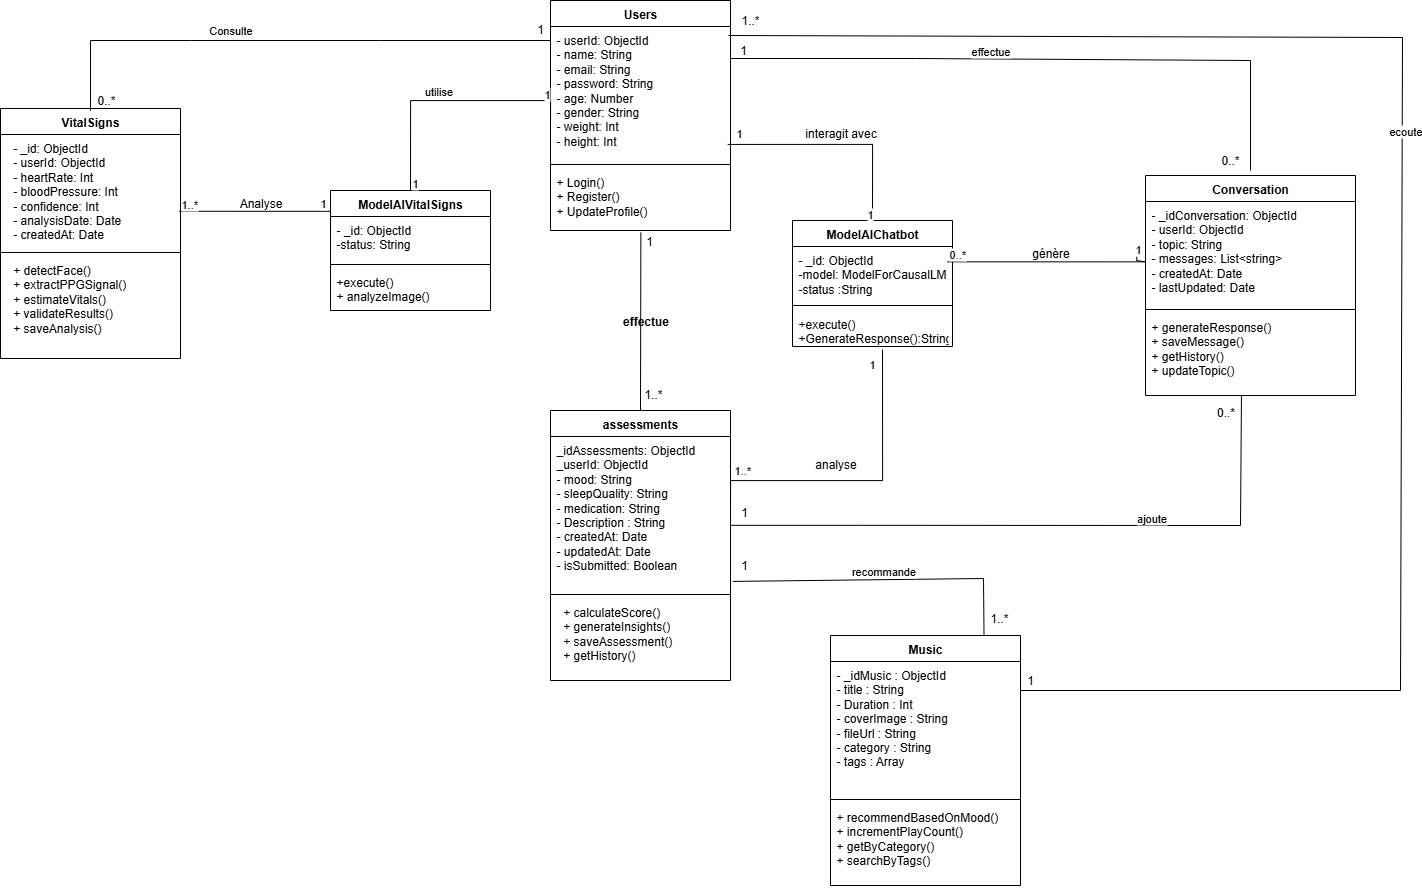
\includegraphics[angle=90, width=0.6\textheight]{Figures/class.png}
    \caption{Diagramme de classe général}
\end{figure}


\section{Conclusion}
Ce chapitre a posé les fondations architecturales et conceptuelles essentielles pour le développement de MindCare-AI. L'adoption du pattern MVC nous offre une séparation claire des responsabilités qui facilite la maintenance et l'évolution du système, tandis que l'architecture modulaire garantit une intégration harmonieuse des composants d'intelligence artificielle avec le socle applicatif.

La modélisation UML complète, incluant le diagramme de cas d'utilisation global et le diagramme de classes, constitue un référentiel de conception partagé qui assure la cohérence entre la vision fonctionnelle et l'implémentation technique. Ces modèles formalisent précisément les interactions utilisateur-système et la structure orientée objet des données, offrant ainsi une base solide pour la réalisation concrète du projet.

Le chapitre suivant entame concrètement l'implémentation de la Release 1 avec le développement progressif du socle applicatif selon la méthodologie agile définie.